\chapter{Programming Languages and Tools}
\label{chap:languages_and_tools}

With the growing distribution of computers and mobile devices, e.g. laptops, smart phones and tablets, the need for programming languages and tools to operate on these machines becomes more and more relevant. Using such tools and languages efficiently, however, often requires much skill and technical aptitude, which in turn takes considerable time and dedication to develop. From the perspective of novice programmers, programming can be extremely hard and overwhelming to get into, especially if they are given no introductory tools and guidance.

This chapter focuses on the distinction between visual and text based programming languages, analysis of both categories, as well as some notable examples. Additionally, these categories are further explored by means of how well they fit in an educational setting.   

\section{Text Based Programming Languages}
\label{sec:text_based_programming_languages}
\todo{Watch the Smalltalk talk, and maybe add something about it here}\\
Text-based programming languages have two distinct subcategories; one is the text-based educational programming languages for novices, and the other is the general purpose programming languages. Event though general purpose programming languages can be used to teach programming to novices, the two categories are distinguished in where the focus of the design has been. This chapter will explore a set of programming languages in both of these categories.

\subsection{Text Based Educational Programming Languages}
This section will provide a description of some different text based educational programming languages and constructs.
\subsubsection{Turtle Programming}
One of the first programming languages that added constructs for learning programming was LOGO. It did not have the constructs from the start, but after 12 seventh-grade students\footnote{From Muzzy Junior High School in Lexington, Massachusetts.} worked with LOGO for a year (1968-1969), Seymour Papert, one of the developers of LOGO, proposed the Turtle as a programming domain that could be interesting to people at all ages. He proposed it since the demonstration had confirmed that LOGO was a learnable \todo{JAIS: Everything is learnable for novices, some stuff is just easier} programming language for novices, but he wanted the demonstration extended to lower grades, ultimately preschool children. Constructs for Turtles was then added to LOGO and has since been widely adopted in other programming languages such as SmallTalk and Pascal, and more recently Scratch\cite{turtle_origin}.

A Turtle can be a visual element on a screen or a physical robot. In Scratch, the Turtle can be any sprite chosen by the user. In LOGO the Turtle is controlled by a set of commands which are:
\begin{itemize}
\item FOWARD X, moves the Turtle X number of Turtle steps in a straight line
\item RIGHT X, turns the Turtle X number of degrees in a clockwise direction
\item LEFT X, turns the Turtle X number of degrees in a counter clockwise direction
\item PENDOWN, makes the Turtle draw
\item PENUP, makes the Turtle stop drawing
\end{itemize}
These commands make up the essence of Turtle programming and the functionality is also present in the other languages which has implemented Turtle programming, maybe using different keywords. Some languages has expanded on these commands, e.g. in Scratch, one can change the color, size and shade of the pen. The commands can be part of user defined functions. Examples could be functions called \emph{SQUARE} or \emph{TRIANGLE} which would draw a square and a triangle respectively using the commands shown. These functions can be part of other functions, e.g. a function called \emph{HOUSE} would use a mix of the commands for correct positioning and then the \emph{SQUARE} and \emph{TRIANGLE} functions to draw the house itself\cite{turtle_func}.

Turtle programming is not only meant as a tool for learning to program. Seymour Papert states that it is meant as an \emph{Object-to-think-with}. This means that it is supposed to give children a way of relating new topics to something they already know. Alan Kay shows an example of this in a talk, where he uses a car sprite (the turtle in this case) to visualize acceleration. He does this by programming a loop for the car that for each iteration makes a circle showing where the car have been and then moves the car forwards to a new position. In each iteration he also increases the distance that the car moves forwards, meaning that the distance between the circles becomes greater and greater, thus visualizing the car accelerating\cite{alan_turtle_video}.

\subsubsection{Small Basic}
Small Basic is a text based programming language with its whole purpose being teaching novices to program. It is not meant as a language one should keep using, but as a tool for learning programming principles and then ``graduating'' to learn more advanced languages. In the developers internal trials they have had success with teaching programming to kids in the ages of 10 and 16, but it is intended for novices in general, so it is not specifically made for that age group\cite{smallbasic_faq}. It is perhaps one of the last languages with this purpose that is still being updated\footnote{With that being said there was a four year hiatus between version 1.0 and 1.1}. It seems as if the focus of teaching programming to novices has changed to visual programming languages, tools for learning existing languages that is meant to be used professionally or languages that are novice friendly, but still meant to be used professionally.

The Small Basic project consist of three pieces: The language itself, an IDE and libraries. This means that one has to use the bundled IDE to program in Small Basic. According to their FAQ\cite{smallbasic_faq}, the language takes inspiration from an early variant of BASIC but is based on the modern .NET Framework Platform. It is much smaller than Visual Basic, it consists of 14 keywords, and supports a subset of the functionality that Visual Basic .NET supports. It does not have a type system and all variables are global and always initialized as to avoid confusion regarding scopes. It is also imperative and does not use or expose beginners to the concept of object orientation.

To learn programming with Small Basic, its website provides a tutorial for getting familiar with the language and the IDE\cite{smallbasic_intro}, and a curriculum. The curriculum can be downloaded for offline use, and teaches general programming topics using Small Basic\cite{smallbasic_curriculum}. Through the introduction one will learn that there are two different window types a program can be run in, either the \emph{TextWindow} which is a regular console, or in the \emph{GraphicsWindow} where graphics can be drawn and so on. So it is possible to create e.g. games in Small Basic. Turtle programming is also supported.

The Small Basic IDE aims to help novices as well. The IDE is made up of different parts, which can be seen in Figure \ref{fig:small_basic_ide}. The first part is the menu bar in the top. It contains a very limited subset of functionality that we are used to see in regular programming IDEs and a Small Basic specific functionality, the Graduate button. The Graduate button can export the code that has been written in Small Basic to Visual Basic so that the developer can keep programming on their project even if they have ``graduated'' to using Visual Basic instead. The second part is the editor itself, where the code is written. The third part is intelliSense and auto complete. It is works the same as in Visual Studio, it shows what is possible to write with a description of what that functionality does. The fourth part is where the error messages are shown and the fifth part shows the properties of a selected element.

\begin{figure}[H]
\begin{center}
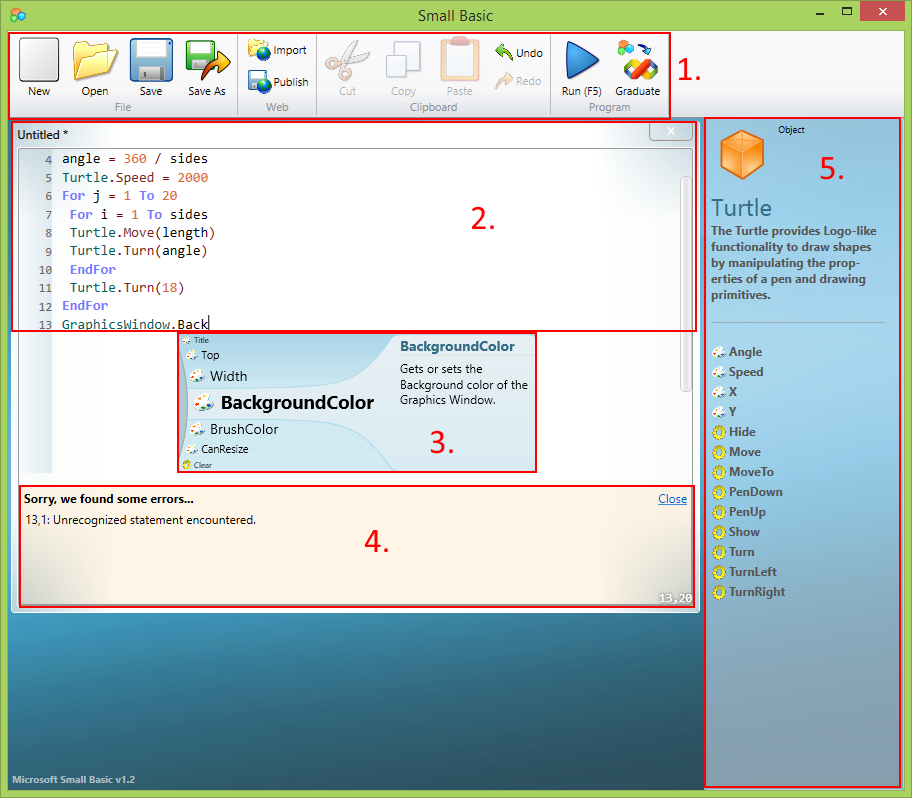
\includegraphics[scale=0.60]{./pics/SmallBasic.png}
\caption{Small Basic IDE}
\label{fig:small_basic_ide}
\end{center}
\end{figure}

\subsection{General Purpose Programming Languages}
This section will provide an overview of some of the general purpose programming languages that has been designed with novices in mind, but still aims to be used as a end-user language. It will also provide an overview of some of the tools used to teach novices to program in languages not specifically designed for novices but as a professional programming language. \todo{We need to discuss terminology further.}

\subsubsection{Programming Languages}
One of the first programming languages designed for novices and to be user friendly is BASIC (Beginner's All-purpose Symbolic Instruction Code). It first appeared in 1964 as a language that would enable students in fields other than science and mathematics to use computers. Since then it became a widely used language and today there are more than 230 different documented dialects of BASIC, among those is Microsoft's Visual Basic.

Another language that was originally designed largely with students in mind was Pascal. It was released in 1970 and aimed to teach students structured programming. However, some early adopters used it far beyond the original intent. This resulted in a lot of work on Pascal and it evolved, both the language itself but also into different dialects, which ended up being designed more towards end-user use rather than an educational tool. Although this meant that the language and dialects became very popular and widely used. The language itself and the dialect called Delphi/Object Pascal is still used today \cite{tiobe}.

A third language that was designed and is still maintained as an easy-to-use general purpose programming language is Quorum. Quorum is an evidence-based programming language. This means that it is updated and changed according to current research on how an easy-to-use programming language should be designed. Some of the team members behind the language host an annual workshop called The Experience Programming in Quorum (EPIQ), which is ``an international professional development workshop for educators to learn the foundational skills necessary to teach students computer science using the Quorum programming language''\cite{quorum_epiq}.

\subsubsection{BlueJ}
BlueJ is a development environment will allows the creation of Java programs quickly and easily. BlueJ has its roots back in the nineties when Michael Kölling developed a pedagogical language and environment called Blue \cite{bluej_overview}. Essentially, BlueJ was initially released as a port of Blue to Java in 1999 and its support continues to this day, thanks to Sun Microsystems and Oracle.

First and foremost, the focus of BlueJ is that its primarily designed for teaching, with good pedagogy in mind. Therefore, many of its characteristics are centered around that notion such as simplicity,interactivity, maturity and innovation. BlueJ has a smaller and simpler interface compared to professional programming environments such as NetBeans or Eclipse with the deliberate intention of not to overwhelm beginners. Additionally, it allows a great deal of interaction with objects e.g. inspecting their values, calling methods on them, invocation of Java expressions without compilation etc. Given that BlueJ is fifteen years old with a solid foundation and full-time team working on it, beginners in programming can easily make use of its technical support. Being a well established environment, BlueJ also has several original features not present in other IDEs such as object bench code, code pad and scope colouring.	

In order to address better the pedagogical side of BlueJ, the BlueJ development team is constantly looking for ways to improve the learning process of programming and make it easier,simpler and more enjoyable. However, this is often not an easy thing to do since there is no real way to measure how good a design decision is \cite{bluej_blackbox}. Having a way to obtain data from its usage will give the team more control over the environment and will benefit the community of BlueJ users as well. Even more, the collected data could be of interest to the wider researcher community and generally people who might be interested in how BlueJ is being used, to much greater benefit. This idea of expanding the amount and type of data collected, while keeping it anonymous, gave fruition to the Blackbox project.

The Blackbox data collection project was announced at the 2012 SIGSE conference in Raleigh,North Carolina,USA.\cite{bluej_blackbox} Initially, with the feedback form attendees, the data collection method was finalised along with some technical details for the whole process. As already mentioned, one of the key features of the project is keeping the data anonymous in order to avoid any ethical and legal complications. The data collection continues to date, as the only condition is to have BlueJ 3.1.0 or newer in order to participate in this research \cite{bluej_blackbox2}.


\todo{Tools for learning}\\
\todo{Add missing sources!}\\

\todo{Remember to summarize text compared to visual programming.}\\
\todo{transition to visual programming}\\
\todo{Why is it the goal to learn these languages? (Look into Intentional Programming)}\\
\todo{Why can't we stick with the educational ones?}\\
\todo{Why don't we begin with these?}\\
\todo{Good thing about text based, is terminology, one learns to talk about programming, e.g. what is a statement?}

%http://dl.acm.org/citation.cfm?id=1227003
%paper of physical programming

%1: page 218
%2: page 11-15
%3: https://www.youtube.com/watch?v=JDpsXWuedVc
%4: http://smallbasic.com/faq.aspx
%5: http://download.microsoft.com/download/9/0/6/90616372-C4BF-4628-BC82-BD709635220D/Introducing%20Small%20Basic.pdf
%6: http://social.technet.microsoft.com/wiki/contents/articles/16982.small-basic-curriculum-online.aspx
%7: http://www.tiobe.com/index.php/content/paperinfo/tpci/index.html
%8: http://quorumlanguage.com/epiq.php
\section{Visual-based Programming Languages}
\label{sec:visual_based_programming_languages}

Traditionally, most programming languages are categorized as text-based because of the way the program logic is written, by making use of a syntax, specific to every language. Therefore, it is often difficult to learn and use a programming language since it requires one to familiarize oneself with the syntax and available constructs first in order to use the language effectively and that takes skill many people lack. 

In order to address the difficulties in learning programming, for the past 25 years \todo{JAIS: Isn't it longer than that? Either way, a cite is needed}, research has been done on the so called “Visual Programming” or “Graphical Programming”, and dozens of visual-based programming languages have been created. This approach, reserved and used in the past primarily for systems design, allows the use of spatial representations in two or more dimensions in the form of blocks and different structures and shapes. Compared to text-based programming where lines of code are used, graphical programming replaces these with visual objects, essentially replacing the textual representation of language components with a graphical one, more suitable for visual learners and intuitive for people with no prior knowledge in programming. The creation of programs in such languages is defined by placement and connection between visual objects where the syntax is encoded within the objects' shapes.  
The main aim of visual programming languages (VPL) and environments, as stated by Koitz ans Slany \cite{KoitzSlany14}, is “\textit{diminishing the syntactical burden and enabling a focus on the semantic aspects of coding}.” VPL try to facilitate end-user programming, both kids and adult novice programming, empowering the creation of new programs, not just their consumption, effectively minimising the distance between the cognitive and computational model.

Currently, there is a wide variety of visual programming languages with varying popularity such as Alice, Greenfoot, Tynker, Scratch, Raptor and many more. From these, Scratch and Alice will be described and analyzed further.

\subsection{Scratch}
Scratch is a visual-based programming environment which allows users to create visually-rich, interactive projects.  Since its inception in 2003, the main goal of its creators has been to address the needs and interests of young people (primarily ages 8 to 16) and make a soft introduction to the world of programming for them. Publicly released in 2007, the project has grown in size and scope, with a dedicated site hosting all its 11 million projects and with a user base of 8 million \cite{scratchstat}.
Given its targeted audience, one of the main design goals of Scratch is the focus on self-directed learning and exploration through tinkering with the different constructs of the language and environment. This combined with the steady increase of its popularity has prompted hundreds of schools and educational organizations to adopt and integrate it into their curriculum \cite{MaloneyResnick10}.

What makes Scratch a sensible choice for people with no prior programming experience is the fact that it has less emphasis on direct instruction than other programming languages. Instead, it focuses on the aspect of learning through self exploration and peer sharing, which breaks the norm of a traditional educational approach.




\section{Comparison}
\label{sec:comparison_text_visual}
As shown in this chapter both text and visual based programming languages has parts of their domain dedicated to learning programming. This is done mostly through tools, be it environments for general purpose programming languages or visual programming languages where the environment can be seen as a part of the language. Both approaches has pros and cons, and these will be explored in this section.

\begin{description}[style=nextline]
\item[Interface Layout] One of the apparent problems with visual programming environments is that a lot of them has multiple elements, e.g. code, available blocks, etc., where each of them requires a slice of the available screen space. This means that a lot more thought should be put into the interface design, where as environments for text-based programming languages can put less focus on it.
\item[Statement Categories] One of the pros of visual programming environments is that they often require a way of dragging e.g. blocks to create functionality. This means that all of the available blocks, or commands in a text based programming language, is always shown and available to the user (it might be split into categories), which gives the user an overview of the possibilities in the language. Text based programming languages lacks in this aspect, as the user often is presented with an empty editor or some tutorial code, which still does not tell the user much about the possibilities. Small Basic is an example where the possibilities are shown through its auto completion, but the user is just presented with a long list and not all of the commands are descriptive in their naming, possibly making it hard to get an overview for a novice.
\item[Writing Speed] One of the pros of text based programming languages is that it is possible to produce code faster compared to visual programming environments. The reason for this is that visual programming environments often are dependent on moving code blocks using the mouse, and if an user wants to make changes to e.g. a function made up of multiple blocks, they have to pull it apart to get to the block they wish to exchange. In text based environments the user has the possibility of using both the keyboard and the mouse when they want to select something, giving the possibility of using the preferred peripheral of the user.
\end{description}

From this we can see that visual based programming is better for novices, since the statement categories help overcome the initial writing block, which novices will run into, while the strength of writing speed is not important for them.
Similarly text-based programming is better for experts as the writing speed can improve their productivity, while they do not have any problems knowing what they can do.